%%
%% This is file `docultexmm.tex', 
%% Documentation for siam multimedia macros for use with LaTeX 2e
%% 
%% December 19, 2013
%%
%% Version 1.0.1
%% 
%% You are not allowed to change this file. 
%% 
%% You are allowed to distribute this file under the condition that 
%% it is distributed together with all of the files in the siam macro 
%% distribution. These are:
%%
%%  siamltexmm.cls (this file)
%%  siam11.clo   (required size option for 11pt papers)
%%  subeqn.clo   (allows equation numbers with lettered subelements)
%%  siam.bst     (bibliographic style file for BibTeX)
%%  docultexmm.tex (documentation file)
%%
%% If you receive only some of these files from someone, please contact: 
%% multimedia@siam.org  
%% 
%% You are not allowed to distribute this file alone. You are not 
%% allowed to take money for the distribution or use of either this 
%% file or a changed version, except for a nominal charge for copying 
%% etc.
%%
%% \CharacterTable
%%  {Upper-case    \A\B\C\D\E\F\G\H\I\J\K\L\M\N\O\P\Q\R\S\T\U\V\W\X\Y\Z
%%   Lower-case    \a\b\c\d\e\f\g\h\i\j\k\l\m\n\o\p\q\r\s\t\u\v\w\x\y\z
%%   Digits        \0\1\2\3\4\5\6\7\8\9
%%   Exclamation   \!     Double quote  \"     Hash (number) \#
%%   Dollar        \$     Percent       \%     Ampersand     \&
%%   Acute accent  \'     Left paren    \(     Right paren   \)
%%   Asterisk      \*     Plus          \+     Comma         \,
%%   Minus         \-     Point         \.     Solidus       \/
%%   Colon         \:     Semicolon     \;     Less than     \<
%%   Equals        \=     Greater than  \>     Question mark \?
%%   Commercial at \@     Left bracket  \[     Backslash     \\
%%   Right bracket \]     Circumflex    \^     Underscore    \_
%%   Grave accent  \`     Left brace    \{     Vertical bar  \|
%%   Right brace   \}     Tilde         \~}

\documentclass[final,leqno,onefignum,onetabnum]{siamltexmm}

\usepackage{amsmath}

\title{Implementation of a lattice Boltzmann method for immiscible multiphase flow simulations using the level set method} 

\author
{Lorenz Hufnagel, Daniel Zint\\
Chair for System-Simulation, Friedrich Alexander Univerit\"at Erlangen-N\"urnberg\\
Cauerstr. 11, 91058 Erlangen, Germany\\
lorenz.hufnagel@studium.uni-erlangen.de\\
daniel.zint@fau.de % ist das so richtig?
}

\begin{document}
\maketitle
\newcommand{\slugmaster}{%
\slugger{siads}{xxxx}{xx}{x}{x--x}}%slugger should be set to juq, siads, sifin, or siims

\begin{abstract}
	We implemented the lattice Boltzmann method for immiscible multiphase flow simulations and combined it with the level set method according to the paper of G. Th\"ommes \cite{Thoemmes}. The level set method is used to calculate the movement of the interface between the two phases. The input for the level set method is computed by the lattice Boltzmann method. We reimplemented the test cases that are mentioned in the paper, to study the method-coupling and its impact on accuracy.
\end{abstract}

\begin{keywords}
	Lattice Boltzmann method,
	Level set method,
	Free surface,
	Multiphase
\end{keywords}

\begin{AMS}\end{AMS}


\pagestyle{myheadings}
\thispagestyle{plain}
%\markboth{TEX PRODUCTION}{USING SIAM'S MM \LaTeX\ MACROS}

\section{Introduction}
%Something about the two-phase problem and some other algorithms that solve it. We could do this according to the presentation-slides.
In engineering the immiscible two-phase flow problem often needs to be considered. For example, bubble dynamics are decisive for the design of chemical reactors. Also fingering in oil recovery is a common two-phase problem.

The two-phase flow problem can be described with the Navier-Stokes equations for two incompressible fluids. To apply them, we distribute our domain into three parts: $\Omega_1$ and $\Omega_2$ describe the two fluids and $\Gamma = \delta\Omega_1 \cap \delta\Omega_2$ is the interface (Fig. \ref{intro_phases}). The material properties in each fluid are constant and the interface is assumed to be sharp. Thus the material properties are discontinuous and the fluids won't mix.

\begin{figure}[h!]
	\flushright
	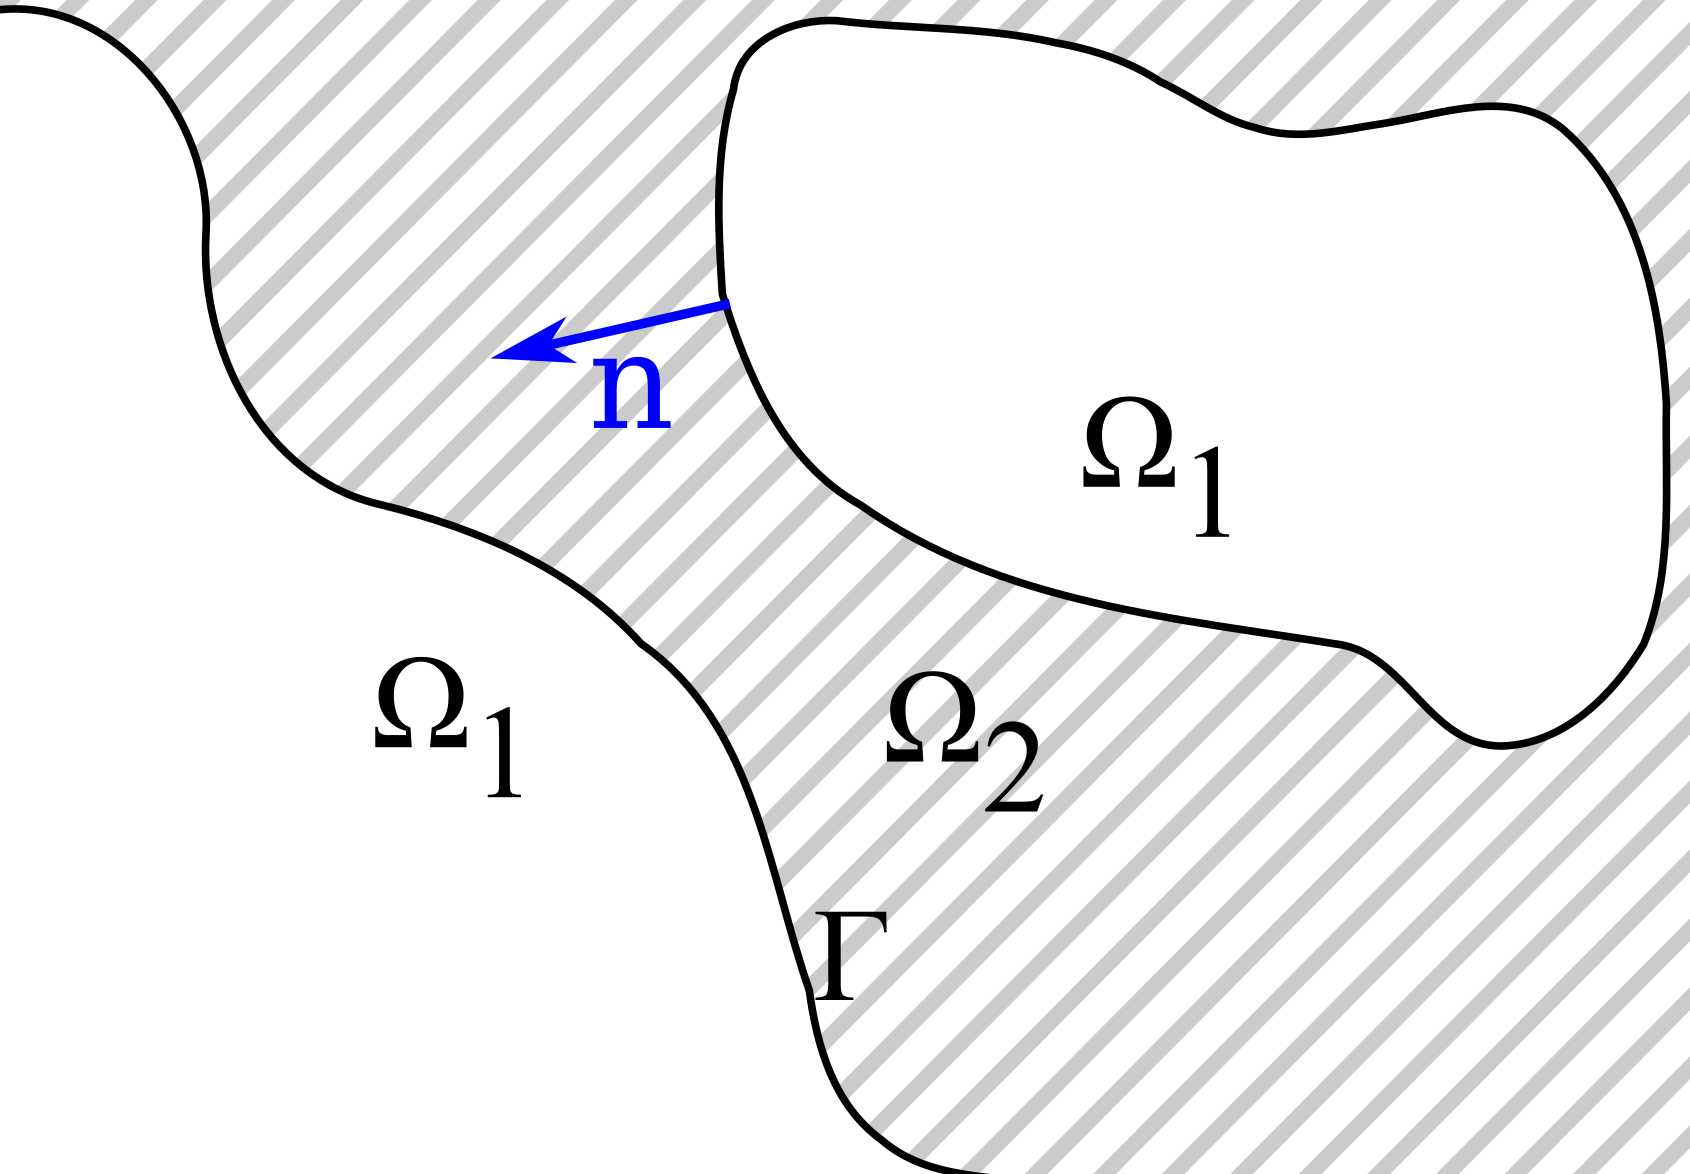
\includegraphics[width=12cm,natwidth=1690,natheight=1174]{skizze.png}
	\caption{Two fluid domains $\Omega_i$ and the interface $\Gamma$ in between}
	\label{intro_phases}
\end{figure}

The evolution of the flow fields within each fluid can be expressed with the incompressible Navier-Stokes equations:
\begin{equation}
	\nabla \cdot  \vec u_i = 0 \text{  in } \Omega_i \text{,}
\end{equation}
\begin{equation}
\frac{\partial \vec u_i}{\partial t} + \left(\vec  u_i\cdot \nabla \right) \vec u_i
=
-\frac{1}{\varrho_i}\nabla p_i + \nu_i \nabla^2 \vec u_i \text{  in } \Omega_i \text{.}
\end{equation}
Here, $u_i$ is the velocity, $p_i$ the pressure, $v_i$ the kinematic viscosity and $\varrho_i$ the mass density.

Furthermore, we need boundary conditions and initial conditions. For our domain-boundaries and the interior we can take for example
\begin{equation}
	u_i(x,t) = 0 \text{, on } \delta\Omega_i \backslash \Gamma \text{,}
\end{equation}
\begin{equation}
	u_i(x,0) = u_{ini,i}(x) \text{, in } \Omega_i \text{.}
\end{equation}
For the interface $\Gamma$ we have the influence of the surface tension and we assume continuity of the velocities within the fluids. Therefore, we get the following jump conditions:
\begin{equation}
	[u] = 0 \text{,  } [T]n = 2 \sigma \kappa n \text{.}
	\label{jumpconditions}
\end{equation}
Here, T is the stress tensor, $\sigma$ the surface tension, and $\kappa$ the curvature of the interface with respect to its normal $n$. Brackets denote the jump of a quantity at the interface: 
$[q](x) = \lim_{\epsilon \rightarrow 0} (q(x - \epsilon n) - (q(x + \epsilon n)) \text{ with } x \in \Gamma$ % I also turned this around, according to [p].
. In Fig. \ref{intro_phases} this would be the jump from $\Omega_1$ to $\Omega_2$. For the other direction the sign changes.

There are different approaches to solve the immiscible two-phase problem. The most spread among these approaches is the colour gradient method of Gunstensen and Rothman \cite{GRcg1,GRcg2,GRcg3}. The downside of this method is that it is only applicable for small density and viscosity differences. Another approach is the concept of {\it interaction potentials} by Shan and Chen \cite{ShanChen1,ShanChen2}. This method actually models miscible fluids and can only approximately describe the behavior of immiscible fluids. Furthermore there are free surface methods which only take one fluid in account for computation (\cite{Koerner}). They work best for big density and viscosity differences.

The method we are presenting uses a hybrid lattice Boltzmann level set method. Thereby the surface motion is calculated by the level set method. The input data for the level set method is given by the lattice Boltzmann method, which is calculated independently for each fluid. This method has the advantage that it has a high accuracy but requires only little memory.

This paper is organized as follows: Section 2 gives an introduction to the numerical methods and the coupling of these. In section 3 we present our results and finally in section 4 we draw a conclusion.

\section{Numerical Methods}
The algorithm uses two numerical methods. Before we show how these can be coupled, we will shortly introduce the numerical methods independently.

\subsection{The Lattice Boltzmann Method}
To solve the incompressible Navier-Stokes equations, we use the lattice Boltzmann method. This method describes the evolution of the particle density $f(\vec{x},\vec{v},t)$ in phase space, with a $(\vec{x},\vec{v})$ as the phase space variables and $t$ as time. The LBM algorithm discretizes with a regular grid in space and with restricted number of velocities adapted to this grid \cite{LBM1,LBM2,LBM3,LBM4}. We use the D2Q9 model in 2D, which has 9 velocity vectors on a plane grid with unit spacing including one zero velocity (Fig. \ref{lbmc_i}). 
\begin{figure}
	\hfill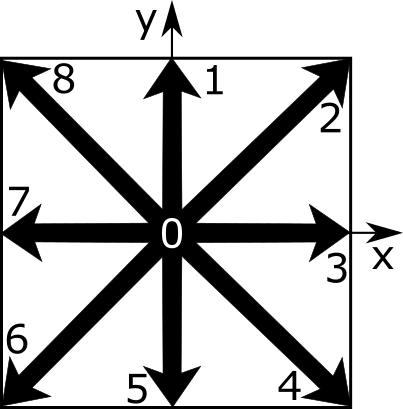
\includegraphics[width=6cm,natwidth=403,natheight=409]{LBMc_i.png}\hspace*{\fill}
	\caption{The vectors of one cell in LBM}
	\label{lbmc_i}
\end{figure}
The vectors are given by the columns of the matrix
\begin{equation}
	c = 
	\begin{bmatrix}
	0 & 0 & 1 & 1 &  1 &  0 & -1 & -1 & -1 \\
	0 & 1 & 1 & 0 & -1 & -1 & -1 &  0 &  1
	\end{bmatrix}
	\text{.}
\end{equation}
The corresponding particle distributions are denoted by $f_i(\vec{x},t) = f(\vec{x},\vec{c_i},t)$. We get the density and velocity from the particle distribution functions with:
\begin{equation}
	\rho(\vec{x},t) = \sum_{i=0}^{8} f_i(\vec{x},t) \text{, } 
	\vec{u} = \sum_{i=0}^{8} f_i(\vec{x},t)\vec{c_i} \text{.}
\end{equation}
For the collision step we use the Bhatnagar-Gross-Krook (BGK) approximation \cite{BGK}
\begin{equation}
	f_i(\vec{x}+\vec{c_i},t+1) = f_i(\vec{x},t) - \frac1\tau(f_i-f_i^{eq}) + G_i \text{.}
\end{equation}
The parameter $\tau$ is the relaxation parameter for the BGK collision operator and controls the kinematic viscosity $\nu = \frac16(2\tau - 1)$. $G_i$ is an additional force like gravity or a magnetic field. In our case we set $G_i = 0$. Furthermore, we use the equilibrium distribution
\begin{equation}
	f_i^{eq}(\rho,\vec{u}) = f_i^*(\rho + 3\vec{c_i} \cdot \vec{u} + \frac92(\vec{c_i} \cdot \vec{u})^2 - \frac32{|\vec{u}|}^2)
\end{equation}
with the corresponding D2Q9 weight factors
$$
f_i^* = \begin{cases} \frac49 \text{,} & i = 0 \\ \frac19 \text{,} & i = 1,3,5,7 \\ \frac{1}{36} \text{,} &  i = 2,4,6,8 \end{cases} \text{.}
$$

The LBM algorithm consists out of the following steps:
\begin{itemize}
	\item[1. ] Collision step: $f_i^+ = f_i - \frac1\tau(f_i - f_i ^{eq}) + G_i$
	\item[2. ] Propagation step: $f_i(\vec{x}+\vec{c_i},t+1) = f_i^+(x,t)$, for interior nodes
	\item[3. ] Boundary conditions: $f_i(\vec{x}+\vec{c_i},t+1) = f_i(\vec{x}+\vec{c_i},t)$, if $\vec{x} \notin \Omega$
\end{itemize}

\subsection{The Level Set Method}
We deal with the movement of the interface between the two fluids by using the level set method. The method captures the surface that represents the interface with a continuous signed distance function which has the interface as the zero level set.

Let $\Gamma_t$ be our interface at time t. Within the level set method, $\Gamma_t$ is the zero iso-surface of the level set function $\varphi$. Thus for $x \in \Gamma_t$ we have $\varphi(x,t) = 0$, in direction of the surface normal we get $\varphi > 0$, and in the other direction we get $\varphi < 0$. For this level set function we get the level set equation of Osher and Sethian \cite{OsherSethian} for the evolution of free surfaces
\begin{equation}
	\varphi_t + v \cdot \nabla \varphi = 0 \text{,}
\end{equation}
with the velocity $v = v(x(t)) = \dot x(t)$ for $x(t) \in \Gamma_t$.

To solve this equation we use the Toolbox of Ian Mitchell \cite{mitchell} for Matlab. This toolbox takes as input the velocity field we get from the lattice Boltzmann method and computes the movement of the interface. The toolbox also provides functions to calculate the normal and the curvature of the surface. We will need this informations for the coupling of the methods.

\subsection{Coupling of LBM and level set method}
The lattice Boltzmann method requires a boundary treatment at the interface which implements the jump conditions (\ref{jumpconditions}). For sake of simplicity, we don't write arrows for every vector, i.e. $\vec{u} \rightarrow u$. One should consider that every position, direction, and velocity is two-dimensional. 

For the coupling, we create a new boundary condition that is based on a simple bounce back type Dirichlet condition. For example, in Fig. \ref{coupling} for a point $x_2 \in \Omega_2$ that is next to the boundary we set
\begin{figure}
	\hfill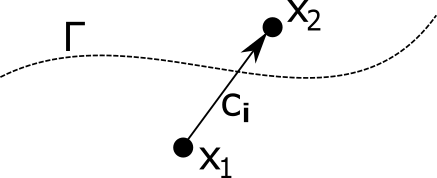
\includegraphics[width=10cm,natwidth=437,natheight=178]{coupling.png}\hspace*{\fill}
	\caption{link between two points in different fluids}
	\label{coupling}
\end{figure}
\begin{equation}
	f_i(x_2,t+1) = f_{i*}^+(x_2,t) + 6hf_i^*c_i \cdot \tilde{u} + R_i \text{.}
\end{equation}
Here, $\tilde{u}$ describes the linear interpolation of the velocity along the direction $c_i$, evaluated at the location $\tilde{x} = x_1 + qc_i = x_2 + (q-1)c_i$ on the interface,
$$
\tilde{u} = qu(x_2,t) + (1-q)u(x_1,t) \text{.}
$$
The additional term $R_i$ ensures the jump conditions of the normal stress and corrects the error terms that are caused by the bounce back treatment. $R_i$ is given as:
\begin{equation}
	R_i = 6 h^2 f_i^* \Lambda_i : A \text{ with } A = -q(1-q)[S] - (q - \frac12)S^{(2)} \text{.}
\end{equation}
We can rewrite the formula in the form
\begin{equation}
	R_i = 6h^2f_i^* \cdot (-q(1-q)\Lambda_i:[S] - (q-\frac12)\Lambda_i:S_2 \text{,}
\end{equation}
with
\begin{equation}
\Lambda_i = c_i \otimes c_i - \frac13 {|c_i|}^2 \mathbf{I} \text{,}
\end{equation}
\begin{equation}
	S_k = -\frac{3}{2\tau h^2} \sum_i c_i \otimes c_i(f_i-f_i^{eq})(t,x_k) \text{.}
\end{equation}
The tensor product is $a \otimes b = ab^T$ and the double contraction $A:B = \mathrm{trace}(AB^T)$. Furthermore, we have
\begin{equation}
	\Lambda_i:[S] = ([S]:n \otimes n)((n \cdot c_i)^2 - {|c_i|}^2/3) + 2([S]:n \otimes t_k)(n \cdot c_i)(t_k \cdot c_i) \text{,}
\end{equation}
with the terms
\begin{equation}
	[S]:n \otimes n =  \frac{1}{2 \bar\mu} ([p] + 2 \sigma \kappa) - \frac{[\mu]}{\bar{\mu}} \bar{S} : n \otimes n \text{,}
\end{equation}
\begin{equation}
	[S]:n \otimes t_k = - \frac{[\mu]}{\bar{\mu}} \bar{S} : n \otimes t_k \text{.}
\end{equation}
Here $n$ is the normal of the interface, $t$ the tangential, $\bar{S} = (S_1 + S_2)/2$ the averaged symmetric velocity gradient, $\kappa$ the curvature, and $\mu$ the dynamic viscosity, with $[\mu] = \mu_2 - \mu_1$ as its jump.
The pressure jump is formulated by
\begin{equation}
	[p] \approx \frac{1}{3 h^2} (\rho(x_2,t)\varrho_2 - \rho(x_1,t)\varrho_1) \text{.}
\end{equation}
What is still missing, is a refill method. Due to the fact that the interface moves, some cells change their fluid type. We use an equilibrium/non-equilibrium refill as it is described in \cite{Caiazzo} that consists out of four steps:
\begin{itemize}
	\item[1] Interpolate density and velocity from interior neighbors
	\item[2] Compute the corresponding equilibrium
	\item[3] Copy the non-equilibrium part from a direct interior neighbor
	\item[4] Reinitialise by adding equilibrium and non-equilibrium parts
\end{itemize}
Suppose we choose an inward pointing direction $c_i$ in a boundary point $x \in \Omega_1$, e.g. the direction of biggest angle with the surface normal. Then the density is interpolated by
\begin{equation}
	\tilde{\rho} = 3\rho(x+c_i,t+1) - 3\rho(x+2c_i,t+1) + \rho(x+3c_i,t+1) \text{.}
\end{equation}
\begin{figure}
	\hfill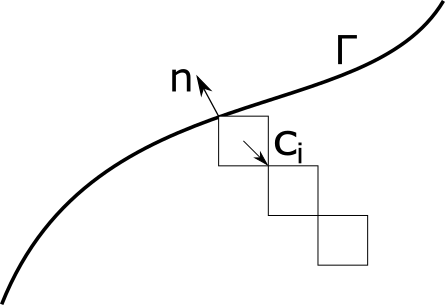
\includegraphics[width=8cm,natwidth=445,natheight=305]{refillmethod.png}\hspace*{\fill}
	\caption{Cells that are used for the refill method}
	\label{refill}
\end{figure}
Figure \ref{refill} shows the cells we use for the interpolation. In \cite{Thoemmes} the velocity is interpolated by using the velocity of the interface. The Ian-Mitchell toolbox does not provide a function to access this value. Therefore, we interpolate the velocity in the same way as we did for the density:
\begin{equation}
\tilde{u} = 3u(x+c_i,t+1) - 3u(x+2c_i,t+1) + u(x+3c_i,t+1) \text{.}
\end{equation}
We can now calculate the new equilibrium $f_i^{eq}(\tilde{\rho},\tilde{u})$ and add it to the non-equilibrium part that we copy from the direct neighbor:
$$f_i(\vec{x},t+1) = f_i^{eq}(\tilde{\rho},\tilde{u}) + f_i^{neq}(x+c_i,t+1) \text{.}$$
We have to repeat the procedure for other fluid.
\begin{figure}
	\hfill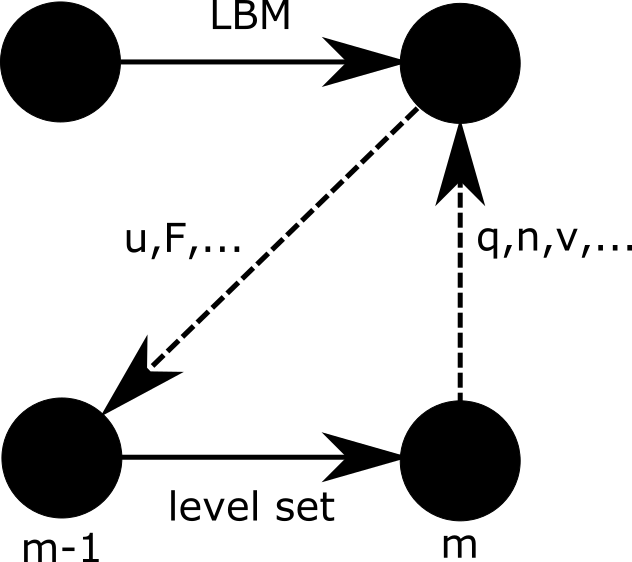
\includegraphics[width=8cm,natwidth=632,natheight=562]{dataexchange.png}\hspace*{\fill}
	\caption{Data exchange between LBM and level set method}
	\label{dataexchange}
\end{figure}

Finally, we can couple the two methods in the following way:
\begin{itemize}
	\item[1.] Create the initial interface $\Gamma_0$
	\item[2.] Run the level set code once to create the surface description for LBM
	\item[3.] Run the LBM using the data from the level set for a prescribed number of steps
	\item[4.] Pass the current velocity field to the level set code and run it for the same number of steps (see Fig. \ref{dataexchange})
	\item[5.] Repeat step 3 and 4 until the end of the simulation.
\end{itemize}

\section{something new what we did / Results}
Present our test case (I think one would be enough) and describe the parameters we have studied. Give graphs that show their impact on accuracy.

\section{Conclusion}

\begin{thebibliography}{1}	

\bibitem{Thoemmes} {\sc G. Th\"ommes, J. Becker}, {\em A lattice Boltzmann method for immiscible multiphase flow simulations using the level set method}, J. Comput. Phys. 228 (2009), 1139-1156

\bibitem{Adalsteinsson} {\sc D. Adalsteinsson, J.A. Sethian}, {\em A fast level set method for propagating interfaces}, J. Comput. Phys. 118 (2) (1995) 269-277

\bibitem{GRcg1} {\sc A.K. Gunstensen, D.H. Rothman, S. Zaleski, G. Zanetti}, {\em Lattice Boltzmann model of immiscible fluids}, Phys. Rev. A 43 (8) (1991) 4320-4327

\bibitem{GRcg2} {\sc A.K. Gunstensen, D.H. Rothman}, {\em Macroscopic modeling of immiscible flows in three dimensions by a lattice Boltzman method}, Europhys. Lett. 18 (2) (1998) 157-161
	
\bibitem{GRcg3} {\sc K. Sankaranarayanan, I.G. Kevrekidies, S. Sundaresan, J. Lu, G. Tryggvason}, {\em A comparative study of lattice Boltzmann and front-tracking finite-difference methods for bubble simulations}, Int. J. Multiphase Flow 29 (1) (2003) 109-116

\bibitem{ShanChen1} {\sc X. Shan, H. Chen}, {\em Lattice Boltzmann model for simulation flows with multiple phases and components}, Phys. Rev. E 47 (3) (1999) 567-603

\bibitem{ShanChen2} {\sc X. Shan, H. Chen}, {\em Simulation of nonideal gases and liquid-gas phase transition by the Lattice Boltzmann equation}, Phys. Rev. E 49 (4) (1994) 2941
	
% Richtige Abkürzung fehlt hier!!!
\bibitem{Koerner} {\sc C. K\"orner, M. Thies, T. Hofmann, N. Th\"urey, U. R\"ude}, {\em Lattice Boltzmann Model for Free Surface Flow for Modeling Foaming}, J. Statistical Physics Vol. 121 (2005) 179-196

\bibitem{LBM1} {\sc S. Chen, G.D. Doolenm}, {\em Lattice Boltzmann method for fluid flows}, Ann. Rev. Fluid Mech. 30 (1998) 329-364

\bibitem{LBM2} {\sc X. He, L.S. Luo}, {\em Lattice Boltzmann model for the incompressible Navier-Stokes equation}, J. Stat. Phys. 88 (1997) 927-944

\bibitem{LBM3} {\sc Sauro Succi}, {\em The Lattice Boltzmann Equation for Fluid Dynamics and Beyond}, Clarendon Press, Oxford, 2001

\bibitem{LBM4} {\sc D.A. Wolf-Gladow}, {\em Lattice-Gas Cellular Automata and Lattice Boltzmann Models}, An Introduction, Springer, 2000

\bibitem{BGK} {\sc P. Bhatnagar, E. Gross, M. Krook}, {\em A model for collision processes in gases: 1. Small amplitude processes in charged and neutral one-component systems}, Phys. Rev. 94 (1954) 511

\bibitem{OsherSethian} {\sc S. Osher, J. Sethian}, {\em Fronts propagating with curvature-dependent speed: algorithms based on Hamlton-Jacobi formulations}, J. Comput. Phys. 79 (1988) 12-49

\bibitem{mitchell}
Mitchell, Ian, A Toolbox of Level Set Methods

\bibitem{Caiazzo} {\sc A. Caiazzo}, {\em Asymptotic analysis of lattice Boltzmann method for fluid-structure interaction problems}, Ph.D. Thesis, Kaiserslautern (Germany) and Pisa (Italy), 2007

\end{thebibliography}


\end{document}
%% end of file `docultexmm.tex'
